\def\year{2020}\relax
\documentclass[letterpaper]{article} % DO NOT CHANGE THIS
\usepackage{aaai20}  % DO NOT CHANGE THIS
\usepackage{times}  % DO NOT CHANGE THIS
\usepackage{helvet} % DO NOT CHANGE THIS
\usepackage{courier}  % DO NOT CHANGE THIS
\usepackage[hyphens]{url}  % DO NOT CHANGE THIS
\usepackage{graphicx} % DO NOT CHANGE THIS
\urlstyle{rm} % DO NOT CHANGE THIS
\def\UrlFont{\rm}  % DO NOT CHANGE THIS
\usepackage{graphicx}  % DO NOT CHANGE THIS
\frenchspacing  % DO NOT CHANGE THIS
\setlength{\pdfpagewidth}{8.5in}  % DO NOT CHANGE THIS
\setlength{\pdfpageheight}{11in}  % DO NOT CHANGE THIS


\pdfinfo{
/Title (BECON: BERT with Evidence from CONceptNet for Common Sense Question Answering)
/Author (Shuailong Liang,Yue Zhang)
}

\setcounter{secnumdepth}{2}
\setlength\titlebox{2.5in}

\title{BECON: \textbf{B}ERT with \textbf{E}vidence from \textbf{CON}ceptNet for Common Sense Question Answering}

% \author{Shuailong Liang \\
%   Singapore University of Technology and Design \\
%   Information System Technology and Design \\
%   Singapore \\
%   \texttt{shuailong\_liang@mymail.sutd.edu.sg} \\\And
%   Yue Zhang \\
%   School of Engineering \\
%   Westlake University \\
%   Hangzhou, China \\
%   \texttt{zhangyue@westlake.edu.cn} \\
% }

\begin{document}

\maketitle

\begin{abstract}

  CommonsenseQA is created by crowdsourcing workers inspired by knowledge graphs on ConceptNet. Solving the task requires the model to have common sense or world knowledge like humans. Current LM-pretrained model such as BERT achieves state-of-the-art performance on the CommonsenseQA dataset, which implies that language models trained on very large corpus may learn some sort of common sense knowledge implicitly. On the other hand, we find that with the availability of the large knowledge graph such as ConceptNet, we can search for helpful evidence to further complement the BERT model. By searching evidences, ranking them, and incorporating them into the BERT model, our single model improves the BERT-large baseline by absolute 1.2\%, and our ensemble model further improves by 3.1\% over the BERT-large baseline.

\end{abstract}

\section{Introduction}

Sit eiusmod laborum ex ipsum laborum sint cillum in minim ea aliqua ad sit. Quis officia deserunt proident Lorem ad magna exercitation ea. Eiusmod ex qui anim officia ex irure ipsum ex sint eu duis sit ipsum. Aliqua aute tempor excepteur deserunt ipsum quis mollit tempor enim ea sunt officia. Est aute enim qui ullamco ad enim sint nisi deserunt ea nulla esse irure. Culpa deserunt esse non pariatur deserunt tempor. Elit pariatur ea aliquip mollit Lorem ipsum aute Lorem aute in commodo velit reprehenderit. Figure~{ref:figure}

Mollit commodo eiusmod fugiat minim veniam minim fugiat. Magna deserunt Lorem officia ullamco. Occaecat irure eiusmod duis mollit occaecat laboris duis nostrud tempor qui irure magna. Sit tempor officia cupidatat anim ipsum commodo laboris amet excepteur labore reprehenderit ea nisi duis.

Ad ex enim esse amet esse ea eiusmod Lorem do. In duis non non exercitation eu incididunt pariatur tempor. Eiusmod nulla ipsum laboris dolor pariatur. Ipsum ea tempor occaecat reprehenderit Lorem veniam do. Et Lorem adipisicing ex nostrud nisi ea anim amet. Aute quis veniam incididunt amet aliqua eu ipsum. Exercitation adipisicing sit dolore elit.

\begin{figure}[t!]
  \centering
  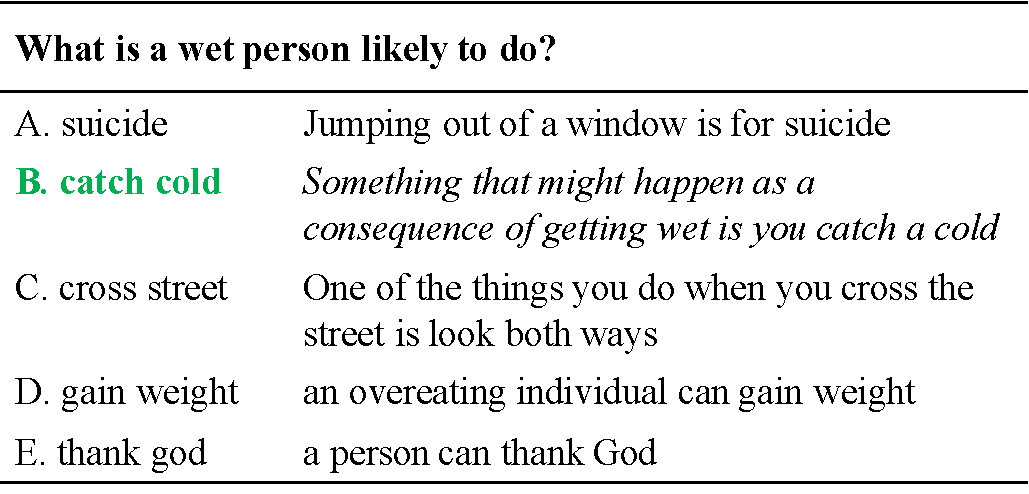
\includegraphics[width=\columnwidth]{figure}
  \caption{A question from CommonsenseQA dataset and its 5 candidate answers with their corresponding top-ranked evidences. The correct answer are in {\bf bold}/green, and the evidence corresponding to the correct answer is it {\it italic}.}
  \label{figure:introdemo}
\end{figure}

Irure sint ipsum nulla reprehenderit velit do quis laborum adipisicing fugiat proident. Consequat aute eiusmod ad proident occaecat nisi eu. Aliqua cupidatat magna sint anim. Culpa deserunt ad ullamco eiusmod voluptate tempor esse fugiat enim mollit in ullamco. Ex mollit do adipisicing amet.
Nostrud nostrud exercitation dolore incididunt minim aliquip ea eu exercitation culpa consequat reprehenderit. Aliquip velit ullamco esse aute exercitation cupidatat irure excepteur. Anim incididunt incididunt ipsum velit non enim eiusmod ipsum laborum veniam proident consequat ex ea. Aliquip sit proident tempor dolor et labore culpa sint. Ex excepteur ad do qui eu eiusmod do in proident officia.

Aute officia qui reprehenderit in nostrud dolore fugiat reprehenderit aute commodo mollit dolor. Aliqua fugiat voluptate commodo mollit non sunt in velit enim voluptate voluptate do ipsum. Non officia do labore aliqua eu eu excepteur adipisicing tempor. Aute eiusmod ipsum commodo in officia mollit.

Ad ex enim esse amet esse ea eiusmod Lorem do. In duis non non exercitation eu incididunt pariatur tempor. Eiusmod nulla ipsum laboris dolor pariatur. Ipsum ea tempor occaecat reprehenderit Lorem veniam do. Et Lorem adipisicing ex nostrud nisi ea anim amet. Aute quis veniam incididunt amet aliqua eu ipsum. Exercitation adipisicing sit dolore elit.

Irure sint ipsum nulla reprehenderit velit do quis laborum adipisicing fugiat proident. Consequat aute eiusmod ad proident occaecat nisi eu. Aliqua cupidatat magna sint anim. Culpa deserunt ad ullamco eiusmod voluptate tempor esse fugiat enim mollit in ullamco. Ex mollit do adipisicing amet.
Nostrud nostrud exercitation dolore incididunt minim aliquip ea eu exercitation culpa consequat reprehenderit. Aliquip velit ullamco esse aute exercitation cupidatat irure excepteur. Anim incididunt incididunt ipsum velit non enim eiusmod ipsum laborum veniam proident consequat ex ea. Aliquip sit proident tempor dolor et labore culpa sint. Ex excepteur ad do qui eu eiusmod do in proident officia.

Aute officia qui reprehenderit in nostrud dolore fugiat reprehenderit aute commodo mollit dolor. Aliqua fugiat voluptate commodo mollit non sunt in velit enim voluptate voluptate do ipsum. Non officia do labore aliqua eu eu excepteur adipisicing tempor. Aute eiusmod ipsum commodo in officia mollit.

\section{Related Work}

Laborum dolor et commodo proident proident consequat. Anim ipsum deserunt non anim deserunt sunt magna mollit cupidatat nostrud. Laborum magna aliquip occaecat aute excepteur consectetur voluptate aute adipisicing tempor labore aliquip. Sunt aliquip ea velit minim elit tempor tempor sit ut dolore adipisicing occaecat voluptate. Velit laborum ullamco ea sunt nisi velit dolore amet sint est irure anim. Duis eu eiusmod elit est esse dolore enim minim.

Eiusmod esse deserunt do irure ut commodo ipsum esse ea enim aliqua ullamco ex. In minim laboris aliqua fugiat esse reprehenderit ipsum officia ad consequat non mollit. Deserunt Lorem eiusmod aliqua laborum ullamco irure eu commodo consequat officia. Ut enim occaecat occaecat tempor amet qui mollit reprehenderit voluptate ad nulla commodo. Minim ea ad incididunt laboris nisi.

Proident eiusmod et irure incididunt elit exercitation ullamco mollit reprehenderit veniam quis. Esse sit ex deserunt exercitation dolore non nostrud eu consectetur laboris quis. Aliquip deserunt minim Lorem elit non et officia in reprehenderit eiusmod non deserunt laborum officia. Ad consequat exercitation nisi anim eu. Amet officia deserunt nostrud sint tempor velit pariatur.

\section{Models}

The best performing model is BERT-large model ~\cite{talmor2018commonsenseqa}

\subsection{Pretrained-BERT with Next Sentece Prediction Head}

BERT-NSP: Select the choice with the highest NSP score with the question. Results are shown in Table~\ref{table:simple_bert_nsp_model}.

\begin{table}[t!]
  \centering
  \begin{tabular}{l c c c c}
  \hline\hline
  {\bf Model}  & {\bf train } & {\bf dev} & {\bf train(S)} & {\bf dev(S)} \\
  \hline
  BERT-base NSP & 35.36 & 39.39 & 71.28 & 71.99 \\
  BERT-large NSP & 38.41 & 40.38 & 73.54 & 73.14 \\
  \hline\hline
  \end{tabular}
  \caption{The result of the BERT-NSP model which selects the choice with the highest NSP score. train(S) and dev(S) corresponds to the {\it SANITY} version of train and dev set, respectively.}
  \label{table:simple_bert_nsp_model}
\end{table}

\subsection{Pretrained-BERT with Finetuning}

For CommonsenseQA task, a question and five candidate answers are given, and one of the five answers is correct. The candidate answers usually consist of one or two words, forming a \textit{concept}. According to ~\cite{talmor2018commonsenseqa}, the best performing baseline model is the BERT-large model finetuned with CQA dataset. Our model is built based on BERT-large model, but also utilizes additional pieces of evidence from ConceptNet, which provides useful information to answer the question.

\subsection{BECON}

Concretely, to use the knowledge in Conceptnet, we first query each candidate answer in ConceptNet to get a list of evidence sentences which may be helpful to answer the question. In order to reduce the noise, we use pretrained BERT with Next-Sentence-Prediction head (BERT-NSP) to rank the evidence sentences and select the top-scored one. An example of the evidence sentences is shown in Figure~\ref{figure:introdemo}. We believe that BERT-NSP is helpful to rank the relevancy of the question and the evidence sentence.

\subsubsection{Evidence Finder}

Each question has 5 candidate answers. According to our analysis, candidate answers are usually one or two words long. We can use ConceptNet API http://api.conceptnet.io/c/en/ to find all the related information related with a word or phrase in the knowledge graph.

\begin{figure}[t!]
  \centering
  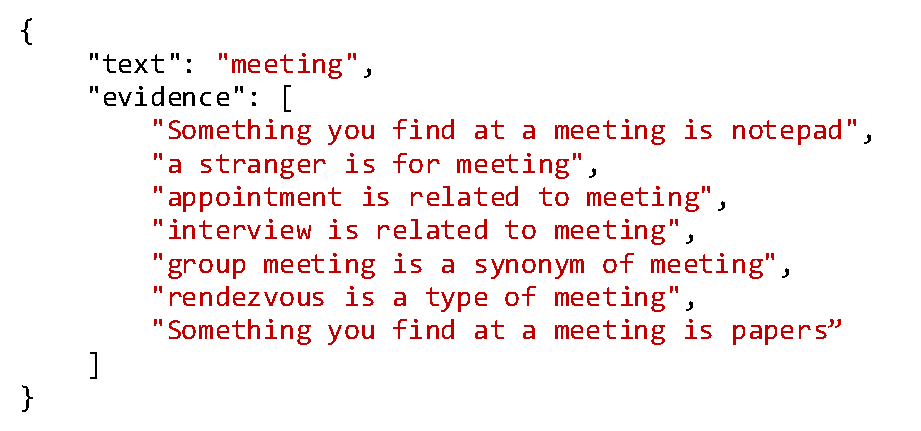
\includegraphics[width=\columnwidth]{evidencefinding.pdf}
  \caption{Subset of evidences from ConceptNet related to the term "meeting".}
  \label{fig:evidencefinding}
\end{figure}

We expect that such evidences may be helpful to answer the question. The problem is, the evidence is too noisy. How to extract useful information? We would like to keep the evidence which is relevant to the question, and discard others. Assume that at most 1 evidence sentence is helpful (which means 0 or 1). We can first rank the evidences and then use the top-ranked evidence (or not).

\subsubsection{Evidence Ranker}

The evidence ranker ranks the evidences according to the relevant scores with the question. We consider some of the very simple rankers:

\begin{itemize}
	\item random: no ranking. Just random shuffle.
	\item jaccard: Jaccard Index is a metrics which consider the words "intersection over union" between question and evidence sentences.
	\item w2v: the cosine distance between the average of pretrained word2vec embeddings of question and evidence sentences.
	\item BERT: use pretrained BERT model along with its Next Sentence Prediction head to determine the relevancy of two sentences.
\end{itemize}


\subsubsection{Evidence Integrator}

As in \cite{talmor2018commonsenseqa}, each question-answer pair is linearized into a delimiter-separated sequence (i.e., "{\tt[CLS]} If ... ? {\tt [SEP]} bedroom {{\tt [SEP]}") and the hidden vector over the {\tt [CLS]} token are used as representation of the choice. For our BECON model, we further concatenate the evidence sentence (i.e., "{\tt [CLS]} If ... ? {\tt [SEP]} bedroom {\tt [SEP]} bedroom is a place for sleeping {\tt [SEP]}"), which may help the model make better decisions.

$${\tt [CLS]} + Q + {\tt [SEP]} + A + {\tt [SEP]}$$
$${\tt [CLS]} + Q + {\tt [SEP]} + A + {\tt [SEP]} + E + {\tt [SEP]}$$

\section{Experiments}

\subsection{Dataset}

\subsection{Experimental Settings}

\subsection{Development Experiments}

\subsubsection{Evidence Rankers}

To have a sense of how the rankers work, we use the ranker to rank all the evidences of the 5 candidate answers. The candidate answer with the top ranked evidence is chosen as the predicted answer. A simple model without training (Naive-Evidence): select the choice with the highest evidence score. The result on train and dev is shown in Table~\ref{table:simple_evidence_model}.

\begin{table}[t!]
  \centering
  \begin{tabular}{l c c c c}
  \hline\hline
  {\bf Ranker}  & {\bf train } & {\bf dev} & {\bf train(S)} & {\bf dev(S)} \\
  \hline
  random & 21.24 & 19.82 & 21.07 & 19.57 \\
  jaccard & 23.12 & 22.44 & 44.43 & 41.28 \\
  w2v & 26.05 & 23.91 & 48.73 & 47.01 \\
  BERT-base & 34.95 & 34.73 & 82.89 & 81.90 \\
  BERT-large & {\bf 36.50} & {\bf 36.86} & {\bf 84.41} & {\bf 82.88} \\
  \hline\hline
  \end{tabular}
  \caption{The result of the Naive-Evidence model which selects the choice with the highest evidence score. train(S) and dev(S) corresponds to the {\it SANITY} version of train and dev set, respectively.}
  \label{table:simple_evidence_model}
\end{table}

There is no dev result in the original paper, but if we assume the dev and test result are close, we can see that the BERT-large NSP model without training is only inferior than BERT-large and GPT which use the CQA dataset to train.

\subsubsection{Evidence Integrator}

Table~\ref{table:becon_pretrain_rankers}

\begin{table}[t!]
  \centering
  \begin{tabular}{l c c}
  \hline\hline
  {\bf Pretrain Modles}  & {\bf Rankers } & {\bf dev}  \\
  \hline
  BERT-base & BERT-base & 56.2 \\
  BERT-base & BERT-large & 57.6 \\
  BERT-large & BERT-base & 61.9 \\
  BERT-large & BERT-large & 62.2 \\
  \end{tabular}
  \caption{BECON with different BERT pretrain models and rankers on dev.}
  \label{table:becon_pretrain_rankers}
\end{table}

The comparision between BERT-base/large rankers show that BERT-large ranker is better. The experiments later all use BERT-large ranker.

Compared with our baseline, the result is a bit lower. This means if we add evidence for each answer candidate, the noise may still overwhelms the useful information.

Table~\ref{table:becon_both}

\begin{table}[t!]
  \centering
  \begin{tabular}{l c c}
  \hline\hline
  {\bf Pretrain Modeds}  & {\bf pooling } & {\bf dev}  \\
  \hline
  BERT-large & max & 63.6 \\
  BERT-large & mean & 64.0 \\
  BERT-large & concat(no pooling) & 64.4 \\
  \end{tabular}
  \caption{BECON w/ w/o evidence combination.}
  \label{table:becon_both}
\end{table}

Table~\ref{table:becon_question}

\begin{table}[t!]
  \centering
  \begin{tabular}{l c c}
  \hline\hline
  {\bf BECON Singale Evidence}  & {\bf dev}  \\
  \hline
  BERT-base & 58.3 \\
  BERT-large & 62.8 \\
  \end{tabular}
  \caption{BECON with single evidence}
  \label{table:becon_question}
\end{table}

\subsection{Results}

The experiment results on CQA test split are shown in Table~\ref{table:final_result}. Our single model outperforms the BERT-large baseline by 1.2\%. Using ensemble technique, our model achieves 59.7\%, outperforms CoS-E~\cite{rajani2019explain} by 1.4\%.

\begin{table}[t]
  \centering
  \small
  \begin{tabular}{l c}
  \hline
  {\bf Model}  & {\bf test F1 } \\
  \hline\hline
  BERT-large~\cite{talmor2018commonsenseqa} & 56.7  \\
  \hline
  CoS-E~\cite{rajani2019explain} & 58.2  \\
  \hline
  BECON  & 57.9 \\
  BECON (ensemble)    & 59.6 \\
  \hline
  \end{tabular}
  \caption{Comparison of the test accurary with literature.}
  \label{table:final_result}
\end{table}

\section{Discussion}

An interesting phenomenon is that BERT NSP without any training on CQA dataset has comparable performance with ESIM + ELMO/glove models on CQA dataset.

\subsection{Error Analysis}

Irure reprehenderit culpa sint fugiat officia excepteur non reprehenderit nulla exercitation laborum. Consectetur laboris consectetur mollit adipisicing excepteur reprehenderit consequat nisi in cillum non. Ipsum sit nulla enim ea ut ex cupidatat labore nisi magna ex. Laboris qui officia laborum excepteur qui sit laborum non incididunt. Adipisicing culpa commodo amet laborum irure fugiat commodo consequat deserunt consectetur ea.

Qui dolor anim eiusmod cillum laboris eu ipsum non quis. Commodo aute nisi et deserunt exercitation ex ad quis ea irure ipsum. Irure ullamco dolor elit eu irure laborum veniam aliquip veniam et ut. Enim labore laborum elit ex duis voluptate do velit aliqua sunt minim labore deserunt. Ut cupidatat nostrud ut labore consectetur do qui esse velit. Nulla Lorem ipsum dolore voluptate minim do. Elit dolore occaecat aliquip adipisicing irure amet.

Reprehenderit id irure minim excepteur mollit cupidatat nostrud. Eu nisi tempor sit deserunt est nostrud quis occaecat aute dolore cupidatat pariatur anim. Incididunt culpa sunt consequat enim eiusmod in ea ad consectetur anim commodo culpa et ullamco. Aliqua minim proident voluptate laborum in sunt. Esse et tempor enim tempor ea et dolore laborum ea exercitation anim. Eiusmod officia aliquip irure amet aliqua anim aliquip.

\subsection{Case Study}

Commodo officia consectetur laboris pariatur enim et eu est id excepteur laborum. Cupidatat dolore ut eu exercitation occaecat aliqua. Dolore do dolor Lorem ex cupidatat id id magna irure. Ad est ut occaecat culpa amet. Cillum mollit labore quis ipsum aliquip tempor ut magna occaecat.

Aliquip veniam laborum consequat ullamco exercitation deserunt. Non veniam quis esse magna eu magna elit tempor sunt do enim excepteur. Est eu consectetur amet qui Lorem.

\section{Conclusion}

We use conceptnet to search for evidence, use BERT to rank them, and use BERT as the base model to train the model with evidence. To alleviate the noise introduced by the evidence, we use BERT to encode both w/ w/o evidence, and let model learn to choose which one contributes more. This model outperforms BERT-large baseline by 0.9\% on dev and +1.2\% on test, which proves the effectiveness of our method. For comparison, salesforce research use human generated explaination to enhance the question, which only outperforms our model by 0.3\%.

NOTE: our submitted model is lower than our best model on dev by 0.4\%. However we cannot resubmit until two weeks later. So if the increase is likewise on test set, we may have comparable results with COS-E by Salesforce Research.

\bibliography{aaai2020}
\bibliographystyle{aaai}
\end{document}
